\documentclass{beamer}
% Class options include: notes, handout, trans
%                        
\usepackage[finnish]{babel}
% Theme for beamer presentation.
\usepackage{beamerthemesplit} 
% Other themes include: beamerthemebars, beamerthemelined,beamerthemetree, beamerthemeplain
\usepackage[utf8]{inputenc}
\usefonttheme{professionalfonts}

\title[Aalto-yliopiston perustieteiden korkeakoulu]{Kysyntäohjautuvan joukkoliikenteen matemaattisia malleja ja algoritmeja}
%\subtitle{Examples of lists, columns and graphics}    % Enter your title between curly braces
\author[L. Häme]{Lauri Häme}                 % Enter your name between curly braces
\institute[Aalto-yliopiston perustieteiden korkeakoulu]{Aalto-yliopiston perustieteiden korkeakoulu}      % Enter your institute name between curly braces
\date{\today}      % Enter the date or \today between curly braces

\usepackage{graphicx}

\begin{document}

% Creates title page of slide show using above information
\begin{frame}
  \titlepage
\end{frame}
%\note{Talk for 30 minutes} % Add notes to yourself that will be displayed when typeset with the notes class option.

\section{Johdanto}
% Creates table of contents slide incorporating all \section and \subsection commands.
%\begin{frame}
%  \tableofcontents
%\end{frame}

\subsection{Johdanto}
\begin{frame}
  \frametitle{Johdanto}   % Insert frame title between curly braces
  \begin{itemize}
    \item 
Kysyntäohjautuva joukkoliikenne = bussi- ja taksipalvelujen välimuoto
\item
Väitöskirjan tärkeimpiä tuloksia ovat älykkäät reitinlaskentamenetelmät
\item
Menetelmiä voidaan joukkoliikenteen lisäksi hyödyntää
rahti- ja lentoliikenteessä, lähetti- ja ruoankuljetuspalveluissa sekä sotilaslogistiikassa
  \end{itemize}
\end{frame}


%\subsection{Problem formulation}
\begin{frame}
  \frametitle{Kysyntä \& tarjonta}   % Insert frame title between curly braces
%  \begin{columns}[c]
%  \column{2.5in}  % slides are 3in high by 5in wide
  \begin{itemize}
\item
Ajoneuvojen reitinlaskenta, ohjauslogiikka
\begin{itemize}
\item
Esim. Kutsuplus
\end{itemize}
\item
Matkustajien matkansuunnitteluongelma
\begin{itemize}
\item
Esim. Reittiopas
\end{itemize}
\item
Taloudellinen tasapaino
\end{itemize}
%  \column{2.5in}


%\framebox{\includegraphics[scale=0.6]{esitys01}}
 
%  \end{columns}
\end{frame}

\section{Reitinlaskenta}
\begin{frame}
  \frametitle{Kysyntäohjautuvan joukkoliikenteen ohjauslogiikka}   % Insert frame title between curly braces
  \begin{columns}[c]
  \column{3.5in}  % slides are 3in high by 5in wide
  \begin{itemize}
    \item 
    Kysyntäohjautuva joukkoliikenne perustuu pienten tai keskisuurten ajoneuvojen (esim. minibussien) joustavaan reititykseen 
    \item
    Asiakkaat voivat tilata matkoja reaaliaikaisesti esim. internet-käyttöliittymällä
    \item
    Ajoneuvojen reitit muodostuvat tilattujen matkojen perusteella
    \item
    Ohjauslogiikalla on kaksi tehtävää:
    \begin{itemize}
    \item
    Ajoneuvon valinta kullekin asiakkaalle
    \item
    Ajoneuvojen reitin optimointi
    \end{itemize}
  \end{itemize}
    \column{1.5in}
\centering

%\framebox{
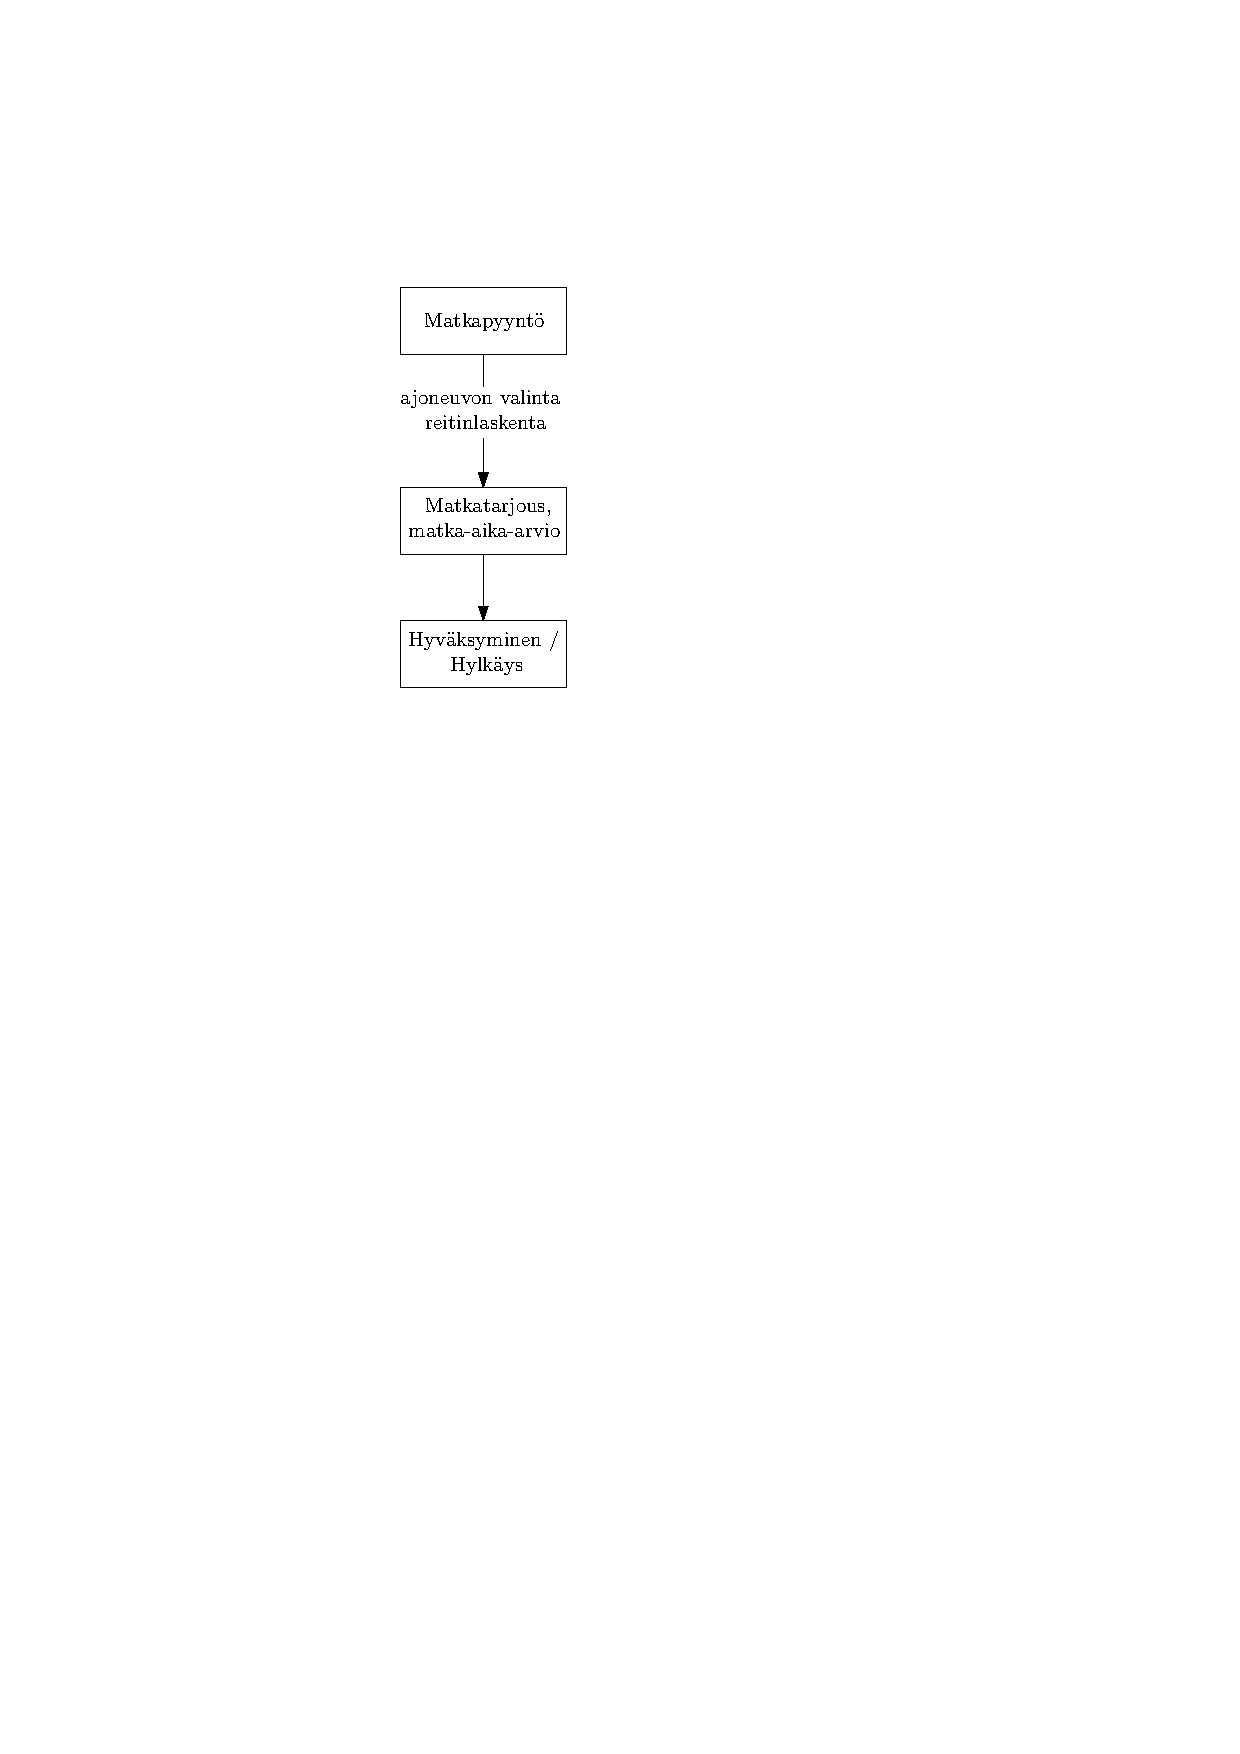
\includegraphics[scale=0.8]{tilauskaavio}
%}
 
  \end{columns}
\end{frame}





\end{document}